\section{Experiments}
\label{sec:experiments}

Our method allows us to identify a family of SDEs that correspond to a given deterministic Gaussian flow model, enabling construction of stochastic samplers with flexible diffusion coefficients.
In our experiments we compare various samplers derived from the corresponding SDEs in \cref{tab:sde_family_table}, using Euler-Maruyama, for a given Gaussian flow model \emph{without any additional training}. 

\begin{figure}[tb]
\centering
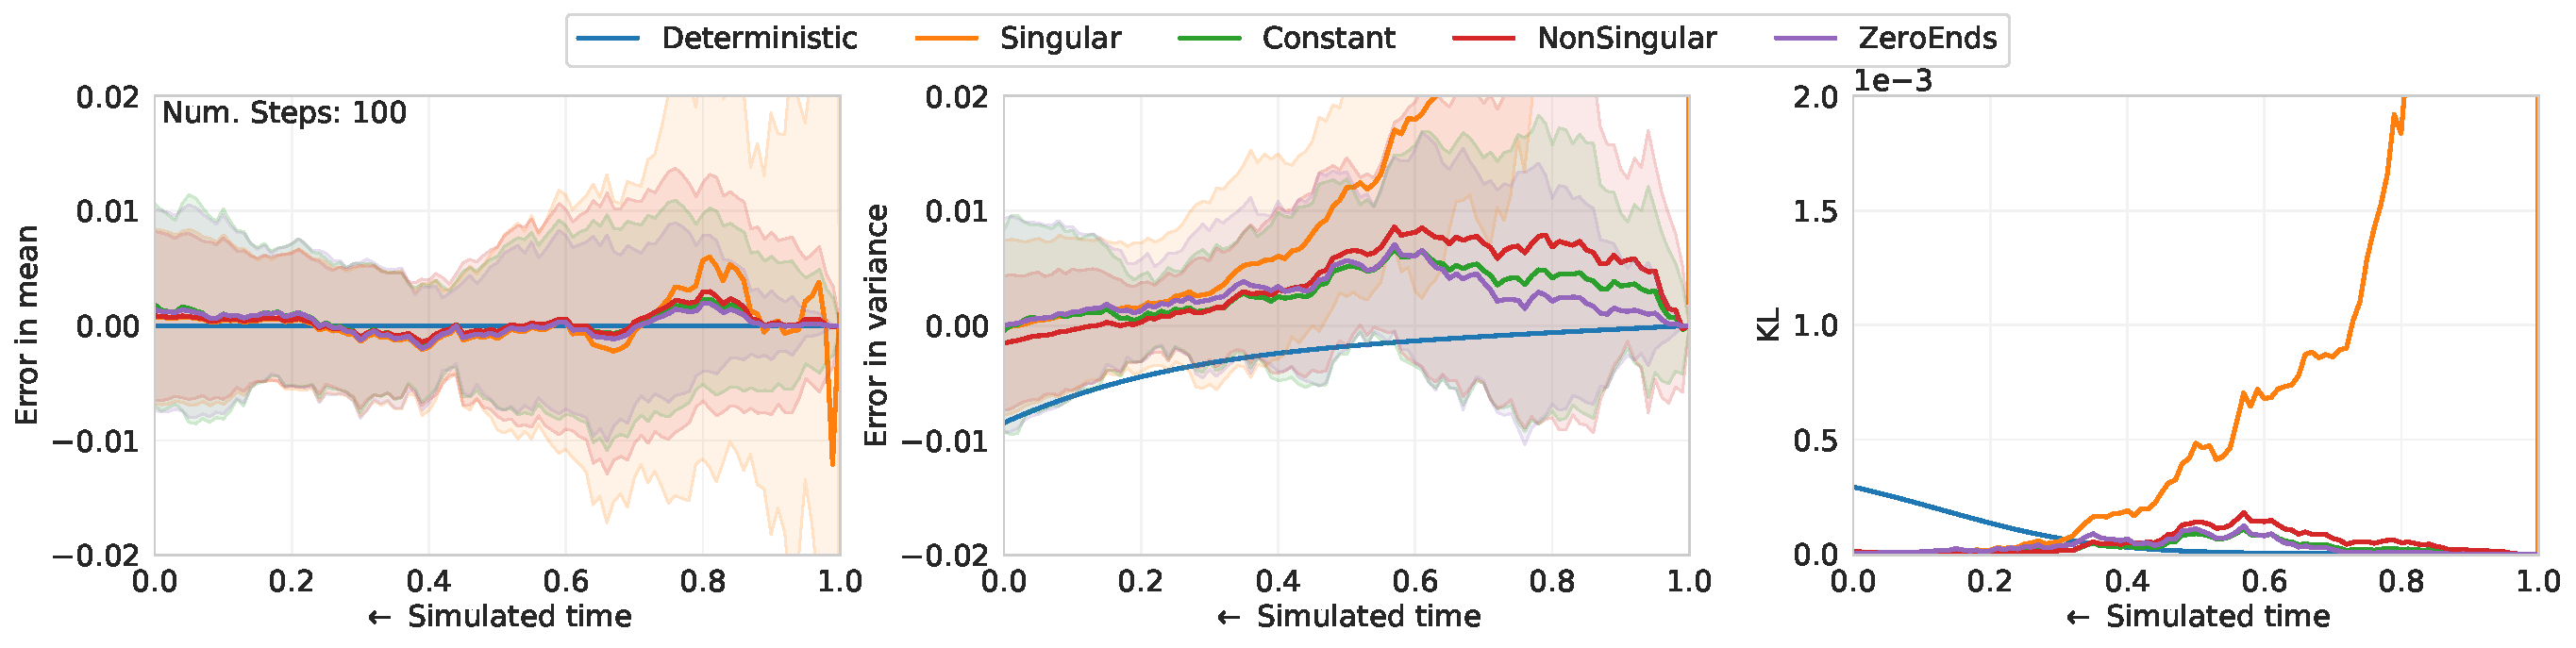
\includegraphics[width=0.99\textwidth]{figs/toy_sampler_comparison_leg_100_kl_2.pdf}
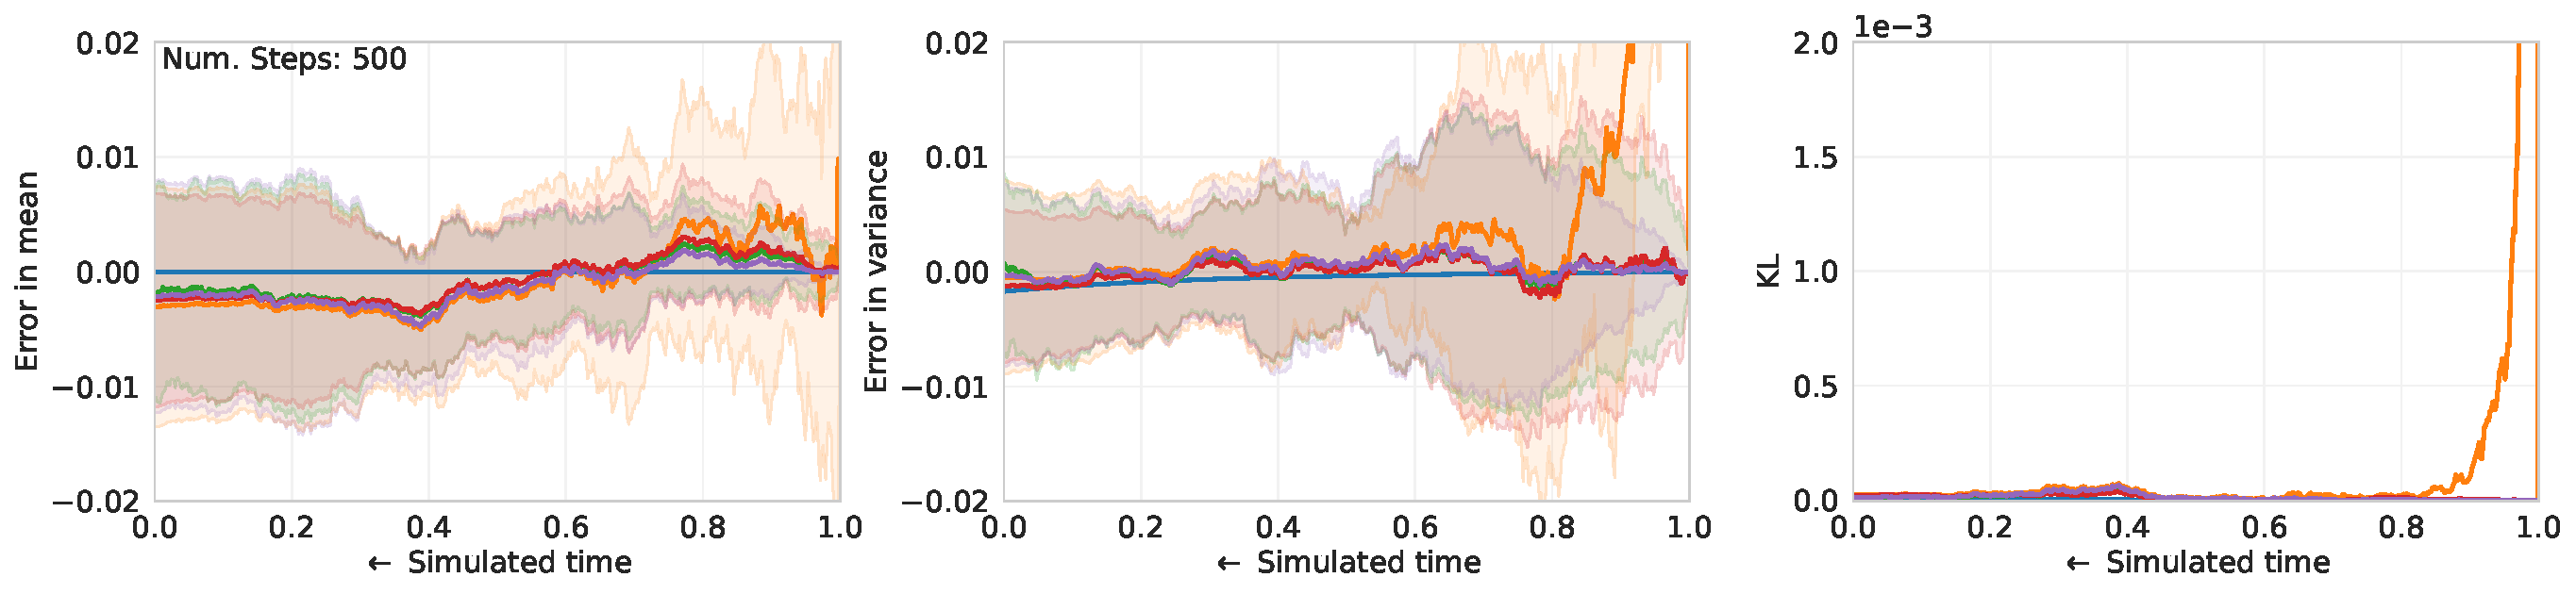
\includegraphics[width=0.99\textwidth]{figs/toy_sampler_comparison_noleg_500_kl_2.pdf}
\caption{%
    \textbf{Stochasticity is most helpful at coarser discretizations.}
    We visualize the effect of coarseness of discretization by sampling for 100 and 500 sampling steps.
    See \cref{fig:toy_samplers} for the same plots at 50 steps, which shows more extreme bias in variance for Deterministic and Singular.
}
\label{fig:toy_steps_eval}
\vspace{-0.3cm}
\end{figure}

\begin{figure}[tb]
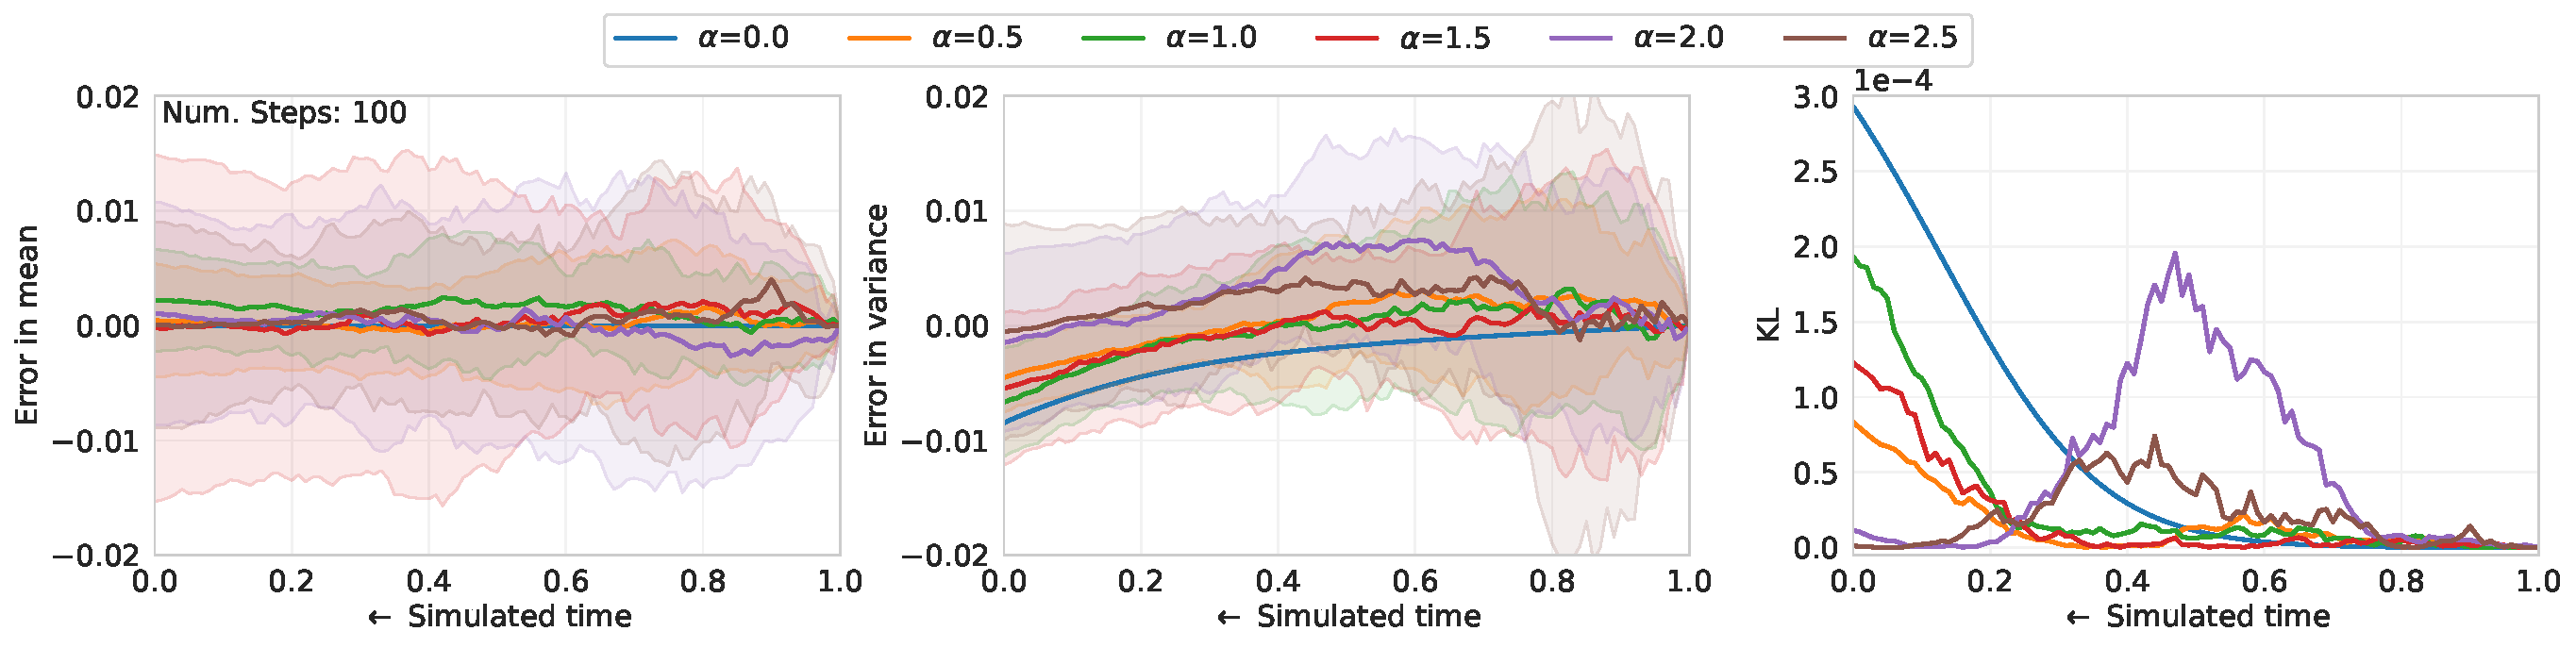
\includegraphics[width=0.99\textwidth]{figs/toy_sampler_comparison_biasvar_nonsingular_kl.pdf}
\caption{%
    \textbf{Stochasticity helps mitigate bias.}
    We plot the error in mean and error in variance for NonSingular for a set of diffusion coefficient scales $\alpha \in \{0.0, 0.5, 1.0, 1.5, 2.0, 2.5\}$. 
    Estimates for variance at $t=0$ improve as $\alpha$ increases, leading to a drop in KL divergence from the true distribution.
    However, with very high $\alpha$ values intermediate marginals develop a bias. 
}
\label{fig:toy_bias_var}
\vspace{-0.4cm}
\end{figure}


\subsection{Comparison on estimating marginal statistics for a two Gaussian toy problem}
\label{sec:guass_experiments}

We start by considering a toy problem where both $p_0$ and $p_1$ are Gaussian.
See \cref{sec:toy_details} for details of the experimental setup and \cref{sec:code} for a JAX~\citep{jax2018github} implementation of NonSingular.

\paragraph{Discretization of deterministic flow leads to bias.}
In \cref{fig:toy_samplers}, with 50 sampling steps, we observe that the estimate for the mean is fairly accurate for all samplers for the entirety of the interval $t \in [0, 1]$.
However, the samplers differ in their behavior for variance.
Deterministic exhibits a noticeable bias and underestimates the variance (with zero variance in its estimate), with the worst estimate at $t=0$.
Stochastic samplers provide noticeably better estimates at $t=0$, but with increased variance.

\paragraph{Stochasticity is most helpful at coarser discretizations.}
In \cref{fig:toy_steps_eval} we study the effect of the number of discretization steps on the different samplers (also see \cref{fig:toy_samplers} for 50 steps).
While mean estimates are accurate for all methods, Deterministic gets increasingly biased for variance estimates as the number of sampling steps is decreased.
Stochastic samplers perform consistently well at various discretization levels for $t=0$, with significantly better estimates for fewer sampling steps.
Note that Singular has very large bias as well as variance closer to $t=1$; those improve with finer discretization.
Since Constant also has a singularity, but only in the drift term $f$, we conclude that the instability is primarily due to the singularity in Singular's diffusion term.

\paragraph{Stochasticity helps mitigate bias.}
In \cref{fig:toy_bias_var} we study the effect of diffusion coefficient scale $\alpha$ on the NonSingular sampler at 100 sampling steps.
Finite discretization introduces a bias in the deterministic sampler (when $\alpha=0$), where the variance is consistently underestimated and is worst at $t=0$.
Increased stochasticity with increasing diffusion coefficient scale ($\alpha>0$) helps mitigate this bias at the cost of increased variance.
This can be seen in the figure with larger $\alpha$ values yielding better estimate of the variance, although with larger variance in the estimate.



\subsection{Comparison of SDEs for rectified flows on ImageNet generation}
\label{sec:imagenet_experiments}

We compare the behavior of various SDEs on the sampling quality for large scale image generation using the ImageNet (2012) dataset~\citep{deng2009imagenet,ILSVRC15}.
We train rectified flow models at two different image resolutions ($64 \times 64$ and $128 \times 128$) and compare their sample quality using the Frechet Inception Distance (FID) metric~\citep{heusel2017gans} for class conditional samples.
See \cref{sec:imagenet_training_details_app} for setup details.
The results show that small but statistically significant differences exist between samplers even for metrics like FID, but the optimal sampler is likely to be application and model specific.

\paragraph{Stochasticity can improve FID.}
In \cref{tab:best_fid} we report the best FID using each SDE in \cref{tab:sde_family_table} for two image resolutions using 300 sampling steps, along with the corresponding diffusion term scale $\alpha$ and one standard deviation confidence interval.
Two key observations stand out:
\textbf{(1)} stochastic samplers tend to produce better FIDs,
and \textbf{(2)} the two non-singular samplers have much better FIDs than Deterministic or Singular.
Note that observation \textbf{(1)} has also been made previously for probability flow ODEs \citep{song2020score}.
The addition of a parameter $\alpha$ to control the strength of the stochasticity while keeping the marginal distribution $p_t$ unchanged (\cref{thm:general}), permits principled post-training optimization of the metrics like FID.

\paragraph{Non-singular samplers work well over a broad range of $\alpha$.}
In \cref{fig:imagenet_fid_alpha,fig:imagenet_fid_alpha_uncropped} we show how the FID varies with $\alpha$ for each sampler for two different image resolution models.
NonSingular and ZeroEnds attain better FID in general and are better behaved over a much larger range of the diffusion coefficient scale $\alpha$ at both resolutions. 
These samplers both have small diffusion coefficients $g(t)$ close to $t=0$; their performance indicates that noise near $t=0$ is particularly harmful.
The low variance of ZeroEnds in comparison to NonSingular indicates that a large diffusion coefficient near $t=1$ tends to introduce variance in the final FID.

\begin{table}[t]
  \caption{%
    \textbf{Stochasticity can improve FID.}
    Comparison of various samplers at their best $\alpha$ values with 300 sampling steps for ImageNet image generation task at two resolutions.
  }
  \label{tab:best_fid}
  \centering
  \begin{tabular}{lLLLL}
    \toprule
    & \multicolumn{2}{c}{$64 \times 64$} & \multicolumn{2}{c}{$128 \times 128$} \\
    \cmidrule(r){2-3}
    \cmidrule(r){4-5}
    Sampler & \text{FID} &  \alpha & \text{FID}  &  \alpha  \\
    \midrule
    Deterministic & 3.07 \pm 0.01 & 0.0  & 5.19 \pm 0.02 & 0.0 \\
    Singular & 3.07 \pm 0.01 & 0.08 & 5.13 \pm 0.04 & 0.14 \\
    Constant $g$ & 2.97 \pm 0.04 & 0.08 & 5.17 \pm 0.05 & 0.1 \\
    NonSingular & \bf{2.95 \pm 0.01} & 0.56 & \bf{4.93 \pm 0.06} & 0.42 \\
    ZeroEnds & \bf{2.95 \pm 0.01} & 0.54 & 5.03 \pm 0.01 & 0.52 \\
    \bottomrule
  \end{tabular}
\end{table}

\begin{figure}[tbp]
\centering
\begin{subfigure}[b]{0.48\linewidth}
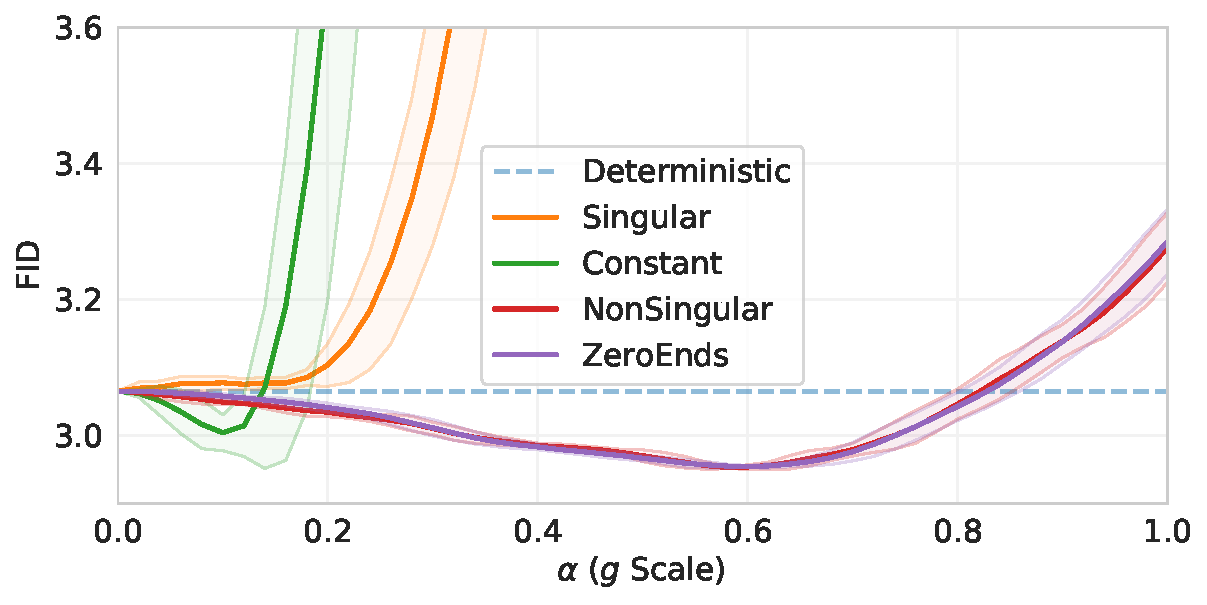
\includegraphics[width=\linewidth]{figs/sampler_scale_comparison_w_64.pdf}
\caption{64 $\times$ 64}
\label{fig:alpha_comparison_crop_64}
\end{subfigure}
\begin{subfigure}[b]{0.48\linewidth}
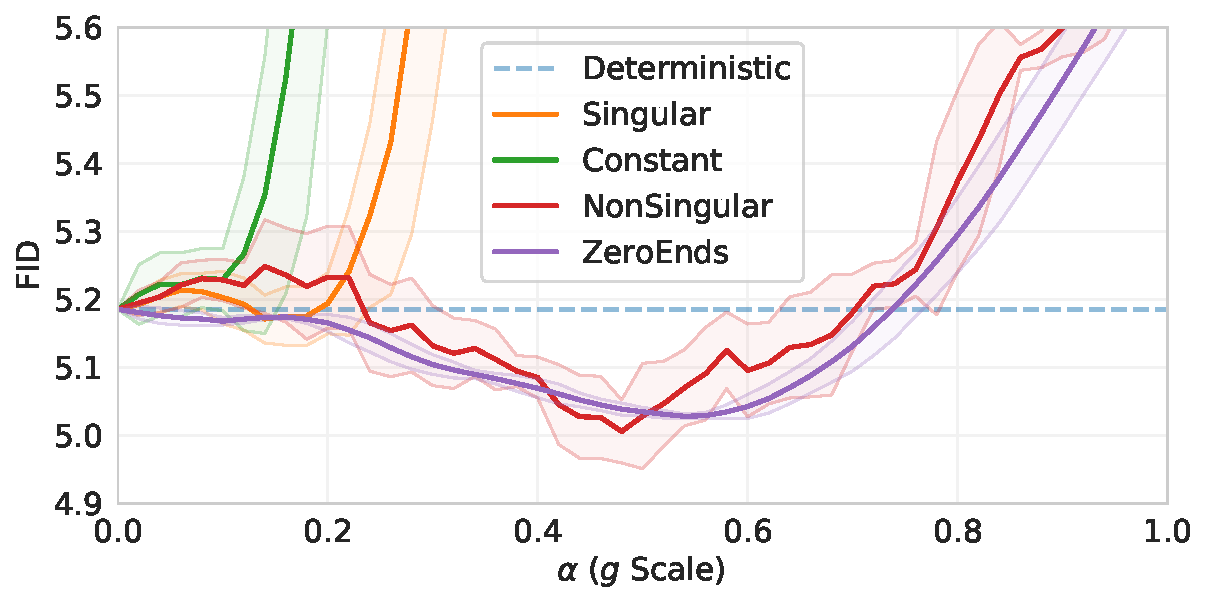
\includegraphics[width=\textwidth]{figs/sampler_scale_comparison_w_128.pdf}
\caption{128 $\times$ 128}
\label{fig:alpha_comparison_crop_128}
\end{subfigure}
\caption{%
    \textbf{Non-singular samplers work well over a broad range of $\alpha$.}
    Plots of FID for each sampler as the diffusion coefficient scale $\alpha$ is increased.
    Note that at $\alpha=0$ all samplers coincide.
    See \cref{fig:imagenet_fid_alpha_uncropped} for a larger range of FIDs.
}
\label{fig:imagenet_fid_alpha}
\end{figure}

\paragraph{Stochasticity makes FID robust to discretization.}
In \cref{fig:imagenet_fid_numsteps} we compare the effect of the number of sampling steps on FID for various samplers at two image resolutions.
We set $\alpha^2$ proportional to the number of sampling steps with the maximum value provided by \cref{tab:best_fid}.
Again the non-singular samplers perform better than Deterministic at all discretization levels.

\paragraph{Stochastic sampling improves diversity at all classifier-free guidance levels.}
In \cref{fig:imagenet_cfg,fig:qual_alpha_vs_lambda} we show samples from NonSingular using classifier-free guidance (\cref{sec:score_function}), varying both $\alpha$ and $\lambda$, the guidance weight.
In all cases, we can see that diversity increases with $\alpha$, and class typicality increases with $\lambda$.

\paragraph{Qualitative comparisons.}
For qualitative comparisons, we visualize a few samples at various diffusion coefficient scales using different SDEs in \cref{fig:constantg_scale,fig:nonsingular_scale,fig:singular_scale}.
All samples in a column are generated by starting at the same draw $x_1 \sim p_1(x_1)$; different columns start from different draws.
Noise scale $\alpha$ gets progressively larger as we move down the rows.
For Constant, we observe that samples get increasingly noisy with increasing $\alpha$ indicating accumulating errors with increasing scale.
The samples from NonSingular look better, as expected from \cref{fig:imagenet_fid_alpha}.
Lastly, samples from Singular change much more rapidly in comparison to the other samplers, indicating that the singularities in the SDE coefficients increase the effect of noise.



\begin{figure}[tbp]
\centering
\begin{subfigure}[b]{0.48\linewidth}
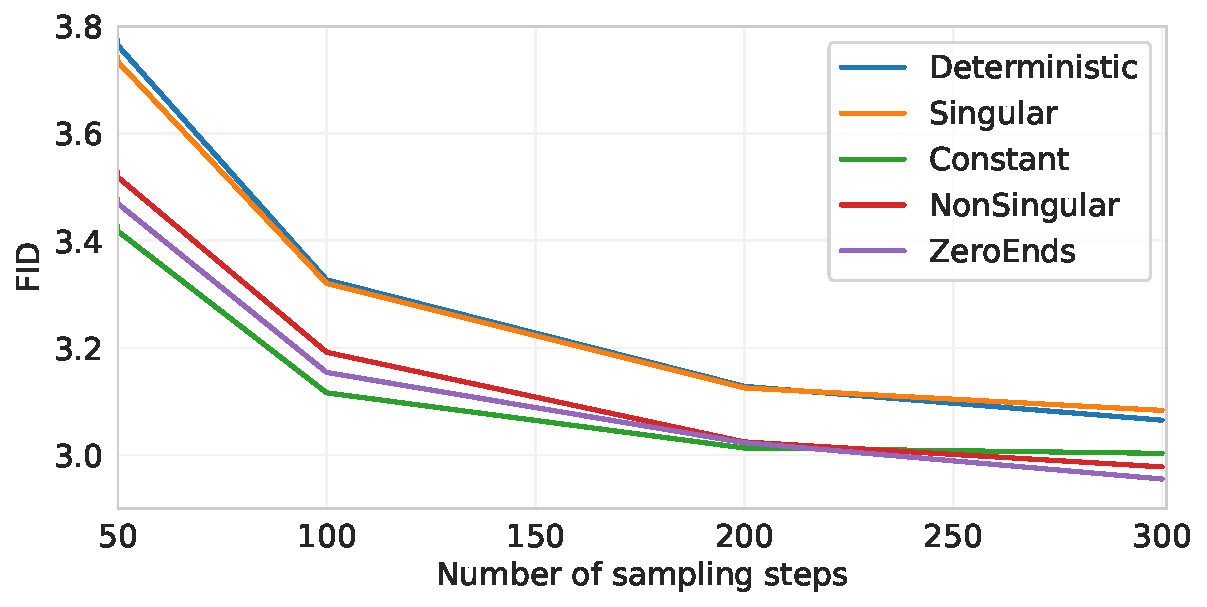
\includegraphics[width=\linewidth]{figs/numsteps_imagenet_fid_w_64.pdf}
\caption{64 $\times$ 64}
\label{fig:imagenet_fid_numsteps_64}
\end{subfigure}
\begin{subfigure}[b]{0.48\linewidth}
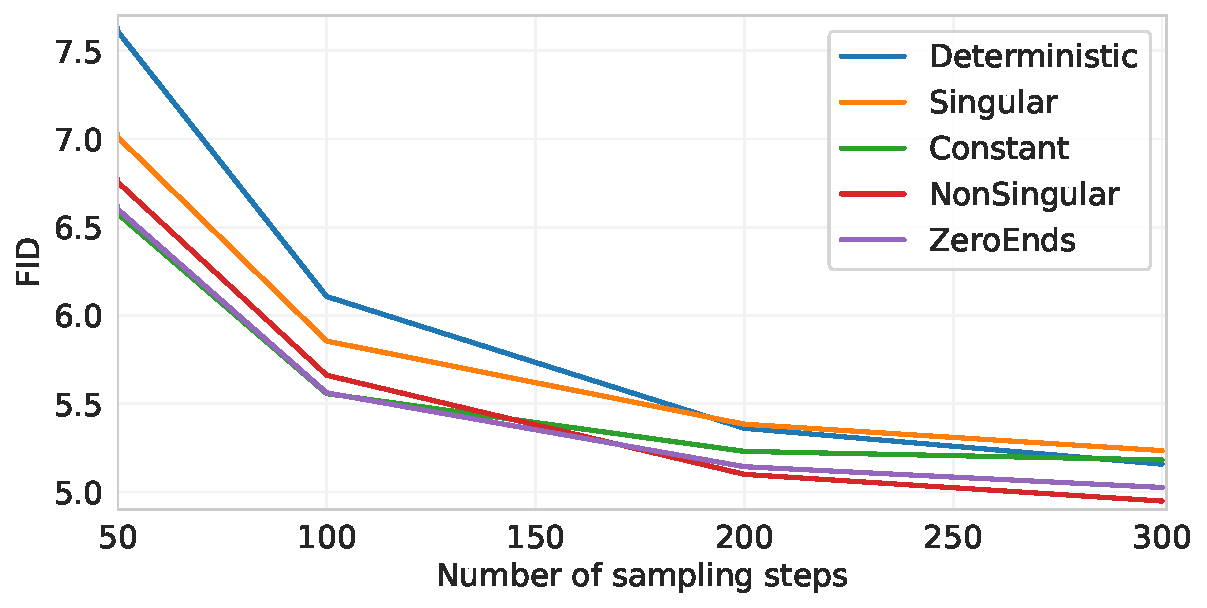
\includegraphics[width=\textwidth]{figs/numsteps_imagenet_fid_w_128.pdf}
\caption{128 $\times$ 128}
\label{fig:imagenet_fid_numsteps_128}
\end{subfigure}
\caption{%
    \textbf{Stochasticity makes FID robust to discretization.}
    We compare the effect of number of sampling steps on FID.
    Deterministic is always worse than the non-singular samplers.
}
\label{fig:imagenet_fid_numsteps}
\vspace{-0.4cm}
\end{figure}

